%%%%%%%%%%%%%%%%%%%%%%%%%%%%%%%%%%%%%%%%%
% Structured General Purpose Assignment
% LaTeX Template
%
% This template has been downloaded from:
% http://www.latextemplates.com
%
% Original author:
% Ted Pavlic (http://www.tedpavlic.com)
%
% Note:
% The \lipsum[#] commands throughout this template generate dummy text
% to fill the template out. These commands should all be removed when 
% writing assignment content.
%
%%%%%%%%%%%%%%%%%%%%%%%%%%%%%%%%%%%%%%%%%

%----------------------------------------------------------------------------------------
%	PACKAGES AND OTHER DOCUMENT CONFIGURATIONS
%----------------------------------------------------------------------------------------

\documentclass{article}

\usepackage{fancyhdr} % Required for custom headers
\usepackage{lastpage} % Required to determine the last page for the footer
\usepackage{extramarks} % Required for headers and footers
\usepackage{graphicx} % Required to insert images
\usepackage{lipsum} % Used for inserting dummy 'Lorem ipsum' text into the template
\usepackage{enumerate}
\usepackage{booktabs}
\usepackage{amsmath}
\usepackage{booktabs}

% Margins
\topmargin=-0.45in
\evensidemargin=0in
\oddsidemargin=0in
\textwidth=6.5in
\textheight=9.0in
\headsep=0.25in 

\linespread{1.5} % Line spacing

% Set up the header and footer
\pagestyle{fancy}
\lhead{\hmwkAuthorName} % Top left header
\chead{\hmwkClass\ (\hmwkTitle)} % Top center header
%%\rhead{\firstxmark} 
\rhead{} % Top right header
\lfoot{\lastxmark} % Bottom left footer
\cfoot{} % Bottom center footer
\rfoot{Page\ \thepage\ of\ \pageref{LastPage}} % Bottom right footer
\renewcommand\headrulewidth{0.4pt} % Size of the header rule
\renewcommand\footrulewidth{0.4pt} % Size of the footer rule

\setlength\parindent{0pt} % Removes all indentation from paragraphs

%----------------------------------------------------------------------------------------
%	DOCUMENT STRUCTURE COMMANDS
%	Skip this unless you know what you're doing
%----------------------------------------------------------------------------------------

% Header and footer for when a page split occurs within a problem environment
\newcommand{\enterProblemHeader}[1]{
\nobreak\extramarks{#1}{#1 continued on next page\ldots}\nobreak
\nobreak\extramarks{#1 (continued)}{#1 continued on next page\ldots}\nobreak
}

% Header and footer for when a page split occurs between problem environments
\newcommand{\exitProblemHeader}[1]{
\nobreak\extramarks{#1 (continued)}{#1 continued on next page\ldots}\nobreak
\nobreak\extramarks{#1}{}\nobreak
}

\setcounter{secnumdepth}{0} % Removes default section numbers
\newcounter{homeworkProblemCounter} % Creates a counter to keep track of the number of problems

\newcommand{\homeworkProblemName}{}
\newenvironment{homeworkProblem}[1][Question \arabic{homeworkProblemCounter}]{ % Makes a new environment called homeworkProblem which takes 1 argument (custom name) but the default is "Question #"
\stepcounter{homeworkProblemCounter} % Increase counter for number of problems
\renewcommand{\homeworkProblemName}{#1} % Assign \homeworkProblemName the name of the problem
\section{\homeworkProblemName} % Make a section in the document with the custom problem count
\enterProblemHeader{\homeworkProblemName} % Header and footer within the environment
}{
\exitProblemHeader{\homeworkProblemName} % Header and footer after the environment
}

\newcommand{\problemAnswer}[1]{ % Defines the problem answer command with the content as the only argument
\noindent\framebox[\columnwidth][c]{\begin{minipage}{0.98\columnwidth}#1\end{minipage}} % Makes the box around the problem answer and puts the content inside
}

\newcommand{\homeworkSectionName}{}
\newenvironment{homeworkSection}[1]{ % New environment for sections within homework problems, takes 1 argument - the name of the section
\renewcommand{\homeworkSectionName}{#1} % Assign \homeworkSectionName to the name of the section from the environment argument
\subsection{\homeworkSectionName} % Make a subsection with the custom name of the subsection
\enterProblemHeader{\homeworkProblemName\ [\homeworkSectionName]} % Header and footer within the environment
}{
\enterProblemHeader{\homeworkProblemName} % Header and footer after the environment
}

%----------------------------------------------------------------------------------------
%	EXPECTATION AND VARIANCE OPERATOR
%----------------------------------------------------------------------------------------
 \newcommand{\E}{\mathrm{E}} 
 \newcommand{\Var}{\mathrm{Var}}
 \newcommand{\Cov}{\mathrm{Cov}}
 \newcommand{\Corr}{\mathrm{Corr}}
 
%----------------------------------------------------------------------------------------
%	NAME AND CLASS SECTION
%----------------------------------------------------------------------------------------

\newcommand{\hmwkTitle}{Problem Set\ \#1} % Assignment title
\newcommand{\hmwkDueDate}{Wednesday,\ February\ 7,\ 2018} % Due date
\newcommand{\hmwkClass}{FIN\ 521} % Course/class
\newcommand{\hmwkClassTime}{2:00pm} % Class/lecture time
\newcommand{\hmwkAuthorName}{Wanbae Park} % Your name

%----------------------------------------------------------------------------------------
%	TITLE PAGE
%----------------------------------------------------------------------------------------

\title{
\vspace{2in}
\textmd{\textbf{\hmwkClass:\ \hmwkTitle}}\\
\normalsize\vspace{0.1in}\small{Due\ on\ \hmwkDueDate}\\
\vspace{3in}
}

\author{\textbf{\hmwkAuthorName}}
\date{} % Insert date here if you want it to appear below your name

%----------------------------------------------------------------------------------------

\begin{document}

\maketitle

%----------------------------------------------------------------------------------------
%	TABLE OF CONTENTS
%----------------------------------------------------------------------------------------

%\setcounter{tocdepth}{1} % Uncomment this line if you don't want subsections listed in the ToC

%%\newpage
%%\tableofcontents
\newpage

%----------------------------------------------------------------------------------------
%	QUESTION 1
%----------------------------------------------------------------------------------------
\begin{homeworkProblem}
	Ratios stated on the problem set are calculated as follows.
	\begin{enumerate}[a.]
		\item Market/Book = Market Capitalization / Book value of equity
		\item Interest coverage = Some measure of income(operating income, EBIT, EBITDA ...) / Interest payments
		\item EV/EBITDA = Enterprise value / EBITDA = Market value of equity + Debt - Cash / EBITDA
		\item Market leverage = Debt / Equity
		\item Current ratio = Current assets / Current liabilities
	\end{enumerate}
	Table \ref{tab:q1-ratios} shows numerical values of ratios calculated by using data from Global Corp's financial statement.
%----------------------------------------------------------------------------------------	
	%% Table of ratios
	\begin{table}[h]
	\centering
	\begin{tabular}{@{}cccccc@{}}
	\toprule
                           & \multicolumn{2}{c}{Definition}          & \multicolumn{3}{c}{Numerical Values} \\ \midrule
	Name of Ratio              & Numerator        & Denominator          & Numerator   & Denominator   & Ratio  \\ \midrule
	\textit{Market/Book}       & Market Cap.      & Book value of equity & 36          & 22.2          & 1.62   \\
	\textit{Interest Coverage} & Operating income & Interest payments    & 10.4        & 7.7           & 1.35   \\
	\textit{EV/EBITDA}         & Enterprise value & EBITDA               & 131.5       & 11.6          & 11.34  \\
	\textit{Market Leverage}   & Debt             & Equity               & 147.9       & 22.2         & 6.66   \\
	\textit{Current Ratio}     & Current assets   & Current liabilities  & 57          & 34.7          & 1.64   \\ \bottomrule
	\end{tabular}
	\caption{Financial ratios of Global Corp. (Unit: million dollars)}
	\label{tab:q1-ratios}
	\end{table}
%----------------------------------------------------------------------------------------	
\end{homeworkProblem}
%----------------------------------------------------------------------------------------	
%----------------------------------------------------------------------------------------
%	QUESTION 2
%----------------------------------------------------------------------------------------
\begin{homeworkProblem}
	\begin{enumerate}[a.]
		\item In this case, \$20 million of cash would be credited, and same amount of long-term debt would be debited. Since the same amount of account in balance sheet have been offset, there is no change in Global's book value of equity.
		\item Inventory would decrease by \$5 million, and there would be also a decrease of book value of equity by \$5 million since retained earning decreases by \$ 5 million.
		\item Since the firm used cash and long-term debt to purchase building, cash amount of \$5 million would be credited, long-term debt amount of \$5 million would be credited, and \$10 million amount of PP\&E would be debited. Since the amount of credited and debited balance sheet account is exactly equal, there is no change in Global's book value of equity.
		\item Because there is no possibility that Global would ever receive payment, there would be a decrease of accounts receivable by \$3 million dollars, as would the book value of equity.
		\item Reduction of cost might affect income statement. It might reduce cost of good sold. However, balance sheet of the firm does not change due to this event.
		\item The balance sheet does not change since the announcement of key competitor is not an economic event.
	\end{enumerate}
\end{homeworkProblem}
%----------------------------------------------------------------------------------------	
%----------------------------------------------------------------------------------------
%	QUESTION 3
%----------------------------------------------------------------------------------------
\begin{homeworkProblem}
\begin{enumerate}[a.]
	\item		%% CASH
	According to the balance sheet of Starbucks for fiscal year 2013, the firm's cash and cash equivalent worth \$2,575.7m, and short-term investments worth \$658.1m. From the 10-K, approximately \$994.4 millions of cash was held in foreign subsidiaries. The majority of short-term investments consisted of US Tresury, commercial paper, corporate bonds, and US Agency securities. Also it is included in certificates of deposit placed through an account registry service.
	\item		%% DEBT
	From the balance sheet of Starbucks, the firm has \$1,299.4m amount of debts.
	\item		%% REARRANGE BALANCE SHEET
	When rearranging balance sheets, liabilities that is a part of operating business is moved to left side, and assets which is non-operating part(such as cash) is moved to right side. Table \ref{tab:prob3-rearrangedsheet} shows the rearranged balance sheet using the rule above.
%----------------------------------------------------------------------------------------
	%% Rearranged Balance Sheet
	\begin{table}[ht]
	\centering
	\begin{tabular}{@{}llll@{}}
	\toprule
	\multicolumn{2}{c}{Operating Accounts}                 & \multicolumn{2}{c}{Financial Accounts}   \\ \midrule
	\textit{Net Working Capital}                       &            & \textit{Net Debt}                    &            \\
	Accounts receivable, net                  & 561.40     & Long-term debt              & 1,299.40   \\
	Inventories                               & 1,111.20   & Other long-term liabilities & 357.70     \\
	Prepaid expenses and other current assets & 287.70     & Cash and cash equivalents   & (2,575.70) \\
	Deferred revenue                          & (653.70)   & Deferred income taxes, net  & (277.30)   \\
	Accounts payable                          & (491.70)   & Short-term investments      & (658.10)   \\
	Accrued litigation charge                 & (2,784.10) & Long-term investments       & (58.30)    \\
	Insurance reserves                        & (178.50)   & Equity and cost investments & (496.50)   \\
	Accrued liabilities                       & (1,269.30) & Deferred income taxes, net  & (967.00)   \\
	TOTAL NET WORKING CAPITAL                 & (3,417.00) & TOTAL NET DEBT              & (3,375.80) \\	\midrule
	\textit{Net Fixed Assets}                          &            & \textit{Shareholder's Equity}        &            \\
	Property, plant and equipment, net        & 3,200.50   & Shareholder's Equity        & 4,482.30   \\
	Other assets                              & 185.30     &                             &            \\
	Other intangible assets                   & 274.80     &                             &            \\
	Goodwill                                  & 862.90     &                             &            \\
	TOTAL NET FIXED ASSETS                    & 4,523.50   &                             &            \\		\midrule
	NET OPERATING ASSETS                      & 1,106.50   & NET BOOK CAPITAL            & 1,106.50   \\ \bottomrule
	\end{tabular}
	\caption{Rearranged Balance Sheet}
	\label{tab:prob3-rearrangedsheet}
	\end{table}
%----------------------------------------------------------------------------------------
	\item		%% ENTERPRISE VALUE
	Enterprise value is calculated as (\textit{Market capitalization + Debt - Excess cash}). It represents market value of the underlying business operations. Since Stabucks' price per share at Sep 29, 2013 is \$55.82, and from 10-K, 749.3 million shares of common stock is outstanding. Therefore, market capitalization of Starbucks is $55.82 \times 749.3 = 41,825.926$ million dollars. From the balance sheet, the amount of cash is 2,575.7 million dollars, and the amount of debt is 1,299.4 million dollars. Therefore, enterprise value of Starbucks is $41,825.926 + 1,299.4 - 2,575.7 = 40,549.626$ million dollars. 
	\item		%% DILUTED EPS
	From the consolidated statements of earnings, diluted EPS is equal to 0.01(unit: million dollars). The number of shares the diluted EPS based on is 762.3 million shares. The reason why the number of diluted shares is different to common stocks is diluted shares contain all convertible securities such as convertible bonds and stock options. Since the denominator is slightly greater than denominator of non-diluted EPS, diluted EPS is slightly less than EPS.
	\item		%% MAIN REASON STARBUCKS MADE LESS PROFIT
	From the income statement, other accounts seems relatively stable, but a huge amount of litigation charge came up. According to Note 15 in 10-K, Kraft commenced a federal court action against Starbucks for termination of distribution arrangement. The arbitrator ordered Starbucks to pay \$2,227.5 million plus prejudgment interest and attorneys' fees. It was reflected on income statement, so Starbucks made less profit than 2012.
	\item		%% P/E RATIO
	P/E ratio is calculated by (\textit{Market capitalization} / \textit{Net income}) or (\textit{Share price} / \textit{EPS}). Therefore, P/E ratio of Starbucks is $\frac{55.82}{0.01} = 5.582$. It can describe whether value of firm is overvalued or undervalued. P/E ratios are commonly used for comparing value of firms in similar industries. Therefore, it is useful to apply P/E ratio to compare Starbucks' value between other's. However, in this case, P/E ratio is too high because of EPS is too low. The main reason of low EPS is litigation charge which is not result of regular operational activity, so high P/E ratio is hardly related to firm's fundamental value. Therefore, for this year, using P/E ratio to compare Starbucks and other competitor is inappropriate.
	\end{enumerate}
\end{homeworkProblem}
%----------------------------------------------------------------------------------------	
%----------------------------------------------------------------------------------------
%	QUESTION 4
%----------------------------------------------------------------------------------------
\begin{homeworkProblem}
	According to the question, expected cash flow stream of the project is as follows.
%----------------------------------------------------------------------------------------	
	%% Cash Flow Table
	\begin{table}[h]
	\centering
	\begin{tabular}{@{}ccccccc@{}}
	\toprule
	\textit{Year}       & \textit{year 0} & \textit{year 1} & \textit{year 2} & \textit{year 3} & \textit{year 4} & \textit{year 5} \\	\midrule
	\textit{Cash flows} & -10             & 5               & 2               & 2               & 2               & 2               \\ \bottomrule
	\end{tabular}
	\caption{Expected Cash Flows} \label{tab:q4-expected cf}
	\end{table}
%----------------------------------------------------------------------------------------	
	The payback period of this project is 4 years because cumulative cash flow from year 1 to year 4 is 11, and that from year 1 to year 3 is 10. That means it takes four years to retake the initial investment. If the required payback period is two years, the project is not accepted since the payback period is larger than required period. Since the cost of capital is given as 10\%, NPV of project is calculated as follows.
	\begin{equation*}	\label{eq:prob4-npv}
	\begin{aligned}
		NPV 		&= -10 + \frac{5}{(1+0.1)} + \frac{2}{(1+0.1)^2} + \frac{2}{(1+0.1)^3} + \frac{2}{(1+0.1)^4} + \frac{2}{(1 + 0.1)^5}	\\
				&= 0.309
	\end{aligned}
	\end{equation*}
	Therefore, the project has a positive NPV, and it means that the project is accepted if we use NPV rule.
\end{homeworkProblem}
%----------------------------------------------------------------------------------------	
%----------------------------------------------------------------------------------------
%	QUESTION 5
%----------------------------------------------------------------------------------------
\begin{homeworkProblem}
	\begin{enumerate}[a.]
	\item
	By using NPV formula, we can plot (cost of capital, NPV) on 2-D space. Figure \ref{prob5-fig:npv_plot} represents plot a function of NPV on r of the project. Decreasing curve on figure 1 represent the NPV curve, and the horizontal line represents NPV = 0, and the vertical line represents cost of capital which makes NPV equals to 0. Therefore, the x-point in which the vertical and horizontal line cross is IRR of the project.
%----------------------------------------------------------------------------------------	
	%% NPV Plot
	\begin{figure}[h]		
	\centering
		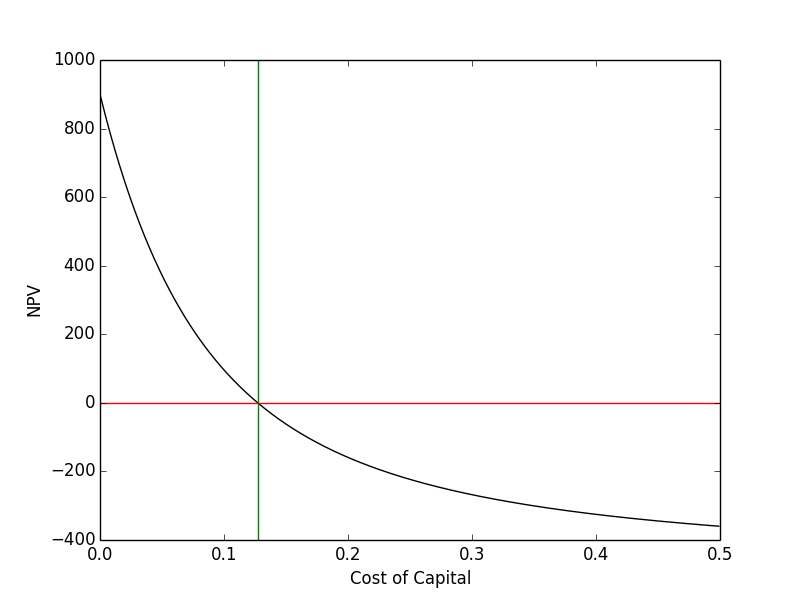
\includegraphics[scale = 0.6]{npv_plot.png} 
		\caption{Plot of NPV}
		 \label{prob5-fig:npv_plot}
	\end{figure} 
%----------------------------------------------------------------------------------------	
	\item
	By some numerical procedures, IRR is calculated as 13\%. It is consistent to figure \ref{prob5-fig:npv_plot} since the x-value of the point in which the vertical and horizontal line cross is larger than 0.1.
%----------------------------------------------------------------------------------------	
	\item
	Since IRR of the project is larger than cost of capital, the purchase is attractive based on IRR decision rule. Also it is attractive based on NPV decision rule because NPV is positive.
%----------------------------------------------------------------------------------------	
	\item
	The decision would change if cost of capital of the project becomes larger than 13\%. Regarding figure \ref{prob5-fig:npv_plot}, we can find that if cost of capital of the project becomes larger than IRR(13\%), NPV of the project would less than 0. It means that it is acceptable to purchase a new cruise ship unless cost of capital of this project becomes greater than 13\%.
	\end{enumerate}
\end{homeworkProblem}
%----------------------------------------------------------------------------------------		
%----------------------------------------------------------------------------------------
%	QUESTION 6
%----------------------------------------------------------------------------------------
\begin{homeworkProblem}
	Regarding event study, NPV of a project can be calculated by market capitalization before an announcement of project times rate of return after the announcement. In order to implement event study, data for market price of share and market capitalization of Bayer and Monsanto was collected. Since it is assumed that it would take about two days for disclosure information to be reflected, price data is collected from Sep 14 to Sep 16. Since the changes of return could be due to changes of whole markets, in order to eliminate that effects, returns of share price is adjusted by subtracting market index(S\&P 500) return. NPVs of Bayer and Monsanto are calculated as -4347.814 million dollars and -1742.227 million dollars, respectively. More details on calculation of NPVs are on table \ref{tab:prob6-npv}.
%----------------------------------------------------------------------------------------
	%% Tables of NPV
	\begin{table}[ht]
	\centering
	\begin{tabular}{@{}ccccc@{}}
	\toprule
	Date                &                       & Bayer     & Monsanto  & S\&P500 \\ \midrule
	2016.9.14           & Closing Price         & 103.4324  & 103.725   & 2125.77 \\
	2016.9.16           & Closing Price         & 98.9536   & 100.51    & 2139.16 \\	\midrule
	\multicolumn{2}{c}{Return}                  & -4.330\%  & -3.100\%  & 0.630\% \\
	\multicolumn{2}{c}{Adjusted Return}         & -4.960\%  & -3.729\%  &         \\		\midrule
	\multicolumn{2}{c}{Market Cap at 2016.9.14 (million dollars)} & 87656.468 & 46715.613 &         \\	\midrule
	\multicolumn{2}{c}{NPV}                     & -4347.814 & -1742.227 &         \\ \bottomrule
	\end{tabular}
	\caption{NPV of M\&A decision}
	\label{tab:prob6-npv}
	\end{table}
%----------------------------------------------------------------------------------------	
	There are some caveats in the analysis. Although I calculated NPV of Bayer and Monsanto by using event study method, the NPV calculated does not guarantee that it is the \textit{real} NPV of M\&A decision. If there is some other information disclosed during the event study period, the NPV obtained above becomes wrong information since other information might affect return of stock price. Of course, such disadvantage can be overcome by choosing short enough period for the analysis. However, if market is not efficient enough, short period makes NPV of firm's decision inaccurate since it takes a certain amount of time to information be reflected. Therefore, because there is a trade-off between reflection of information and accuracy of effect, choosing appropriate period is important.
\end{homeworkProblem}
%----------------------------------------------------------------------------------------	
%----------------------------------------------------------------------------------------
%	QUESTION 7
%----------------------------------------------------------------------------------------
\begin{homeworkProblem}
	From the perspective of capital budgeting, interest expense is ignored when calculating free cash flows. It is because we want to separate the investment and financial decisions.  In order to calculate the free cash flow, the first thing have to do is calculating incremental earnings. It is calculated as \textit{Incremental EBIT}(Incr. Revenues - Incr. Cost - Incr. Depreciation)  $\times$ \textit{(1 - Marginal tax rate)}. After that, make some adjustments to the incremental earning calculated before. Although the amount of depreciation is subtracted when calculating incremental earning, it is not an actual cash outflow. Therefore, we have to add depreciation again. However, it is incorrect not to subtract depreciation when calculating incremental earning because depreciation affects to the amount of tax. Hence, subtraction-and-addition procedure should be applied. Then, the amount of capital expenditure should be subtracted. It is because capital expenditure is actual cash outflow for the project, but it is not captured in income statement. Finally, the amount of changes in net working capital should be subtracted because an increase of net working capital ties up cash. Table \ref{tab:prob7-calcfcf} shows calculation of free cash flow of Cellular Access for this year. The free cash flow of Cellular Access for this year is calculated as 40 million dollars.
%----------------------------------------------------------------------------------------		
\begin{table}[ht]
\centering
\begin{tabular}{@{}cc@{}}
\toprule
Account Subject                 & Value(million dollars) \\ \midrule
EBIT                            & 250   \\
Tax Expense                     & 100   \\ \midrule
Incremental Earnings            & 150   \\
Depreciation                    & 100   \\
Capital Expenditure             & 200   \\
Increase of Net Working Capital & 10    \\ \midrule
Free Cash Flow                  & 40    \\ \bottomrule
\end{tabular}
\caption{Calculation of Free Cash Flow}
\label{tab:prob7-calcfcf}
\end{table}
\end{homeworkProblem}
%----------------------------------------------------------------------------------------	
%----------------------------------------------------------------------------------------
%	QUESTION 8
%----------------------------------------------------------------------------------------
\begin{homeworkProblem}
	\begin{enumerate}[a.]
	\item
	The asset beta is calculated by $\beta_a = w_d \beta_d + w_e \beta_e$, where $\beta_a, \beta_d$, and $\beta_e$ denotes asset beta, debt beta and equity beta, respectively, and $w_d$ and $w_e$ denotes ratio of debt and equity to total amount of debt and equity, respectively. Since the stock price of Thurbinar is \$20 per share and there are 15 million shares outstanding, the market capitalization of firm is $20 \times 15 = 300$ million dollars. Assuming the firm has no cash, the ratio of debt and equity is calculated as $w_d = \frac{100}{300 + 100} = 0.25$ and $w_e = \frac{300}{300 + 100} = 0.75$. Since $\beta_d = 0$ and $\beta_e = 1$, the asset beta of the firm is $\beta_a = 0.25 \times 0 + 1 \times 0.75 = 0.75$. Therefore, by CAPM the asset cost of capital of this firm is $r_a = r_f + \beta_a(r_{mkt} - r_f) = 0.04 + 0.75 \times 0.05 = 7.75\%$
	\item
	By CAPM, $r_e = r_f + \beta_e(r_{mkt} - r_f) = 0.04 + 1 \times 0.05 = 0.09$, and since debt beta of the firm is 0, $r_d$ is equal to risk-free rate, 0.04. Since $w_e = 0.75$ and $w_d = 0.25$, $r_a = w_e r_e + w_d r_d = 0.75 \times 0.09 + 0.25 \times 0.04 = 0.0775 = 7.75\%$.
	\end{enumerate}
\end{homeworkProblem}
\end{document}